%Dies ist die Hauptseite des Dokumentes. Es werden u. a. alle Kapitel,
%Einstellung im Header eingebunden.  Veränderungen müssen in folgenden Dateien
%vorgenommen werden:
      %- Layout.tex
      %- newComments.tex
      %- Titelseite
      %- Versionsübersicht
      %- einzelne Kapitel (evtl. erweitern)



% Definition von globalen Parametern, die derzeit auf der Titelseite und in der
% Kopfzeile verwendet werden. Der in <> gesetzte Text ist zu verändern.

\newcommand{\praktikumTitel}{Ingenieursmäßige Konstruktion, Simulation und Visualisierung von Achterbahnen }
\newcommand{\projektTitel}{Achterbahnsimulator}


%Hier sind alle Einstellungen enthalten, die sich auf das Seiten- und
%Dokumentenlayout beziehen

\documentclass[
  11pt,                % Schriftgröße
  DIV12,
  german,              % für Umlaute, Silbentrennung etc.
  oneside,             % einseitiges Dokument
  titlepage,           % es wird eine Titelseite verwendet
  halfparskip,         % Abstand zwischen Absätzen (halbe Zeile)
  normalheadings,      % Größe der Überschriften verkleinern
  tablecaptionabove,   % Beschriftung von Tabellen unterhalb ausgeben
  final                % Status des Dokuments (final/draft)
]{scrreprt}            %


%------Ändern von Schriftschnitten - (Muss ganz am Anfang stehen !) ------------
\usepackage{fix-cm}

%------Umlaute -----------------------------------------------------------------
%   Umlaute/Sonderzeichen wie äüöß können direkt im Quelltext verwenden werden.
%    Erlaubt automatische Trennung von Worten mit Umlauten.
\usepackage[T1]{fontenc}
\usepackage[utf8]{inputenc}

%------Anpassung der Landessprache----------------------------------------------
\usepackage{ngerman}

%------Einfache Definition der Zeilenabstände und Seitenränder------------------
\usepackage{geometry}
\usepackage{setspace}

%------Schriftgrößenanpassung von einzelnen Textpassagen------------------------
\usepackage{relsize}

%------Trennlinien in Kopf- und Fusszeile
\usepackage[headsepline, footsepline, ilines]{scrpage2}

%------Grafiken-----------------------------------------------------------------
\usepackage{graphicx}

%------Packet zum Sperren, Unterstreichen und Hervorheben von Texten------------
\usepackage{soul}

%------ergänzende Schriftart----------------------------------------------------
\usepackage{helvet}

%------Lange Tabellen-----------------------------------------------------------
\usepackage{longtable}
\usepackage{array}
\usepackage{ragged2e}
\usepackage{lscape}

%------PDF-Optionen-------------------------------------------------------------
\usepackage[
  bookmarks,
  bookmarksopen=true,
  colorlinks=true,
  linkcolor=black,        % einfache interne Verknüpfungen
  anchorcolor=black,      % Ankertext
  citecolor=black,        % Verweise auf Literaturverzeichniseinträge im Text
  filecolor=black,        % Verknüpfungen, die lokale Dateien öffnen
  menucolor=black,        % Acrobat-Menüpunkte
  urlcolor=black,         % Farbe für URL-Links
  backref,                % Zurücktext nach jedem Bibliografie-Eintrag als
                          % Liste von Überschriftsnummern
  pagebackref,            % Zurücktext nach jedem Bibliografie-Eintrag als
                          % Liste von Seitenzahlen
  plainpages=false,       % zur korrekten Erstellung der Bookmarks
  pdfpagelabels,          % zur korrekten Erstellung der Bookmarks
  hypertexnames=false,    % zur korrekten Erstellung der Bookmarks
  linktocpage             % Seitenzahlen anstatt Text im Inhaltsverzeichnis
                          % verlinken
  ]{hyperref}



      % enthält eingebundene Packete

%------Seitenränder-------------------------------------------------------------
\geometry{verbose,                     % zeigt die eingestellten Parameter beim
                                       % Latexlauf an
      paper=a4paper,                   % Papierformat
      top=25mm,                        % Rand oben
      left=25mm,                       % Rand links
      right=25mm,                      % Rand rechts
      bottom=45mm,                     % Rand unten
      pdftex                           % schreibt das Papierformat in die
                                       % Ausgabe damit Ausgabeprogramm
                                       % Papiergröße erkennt
  }

%Seitenlayout
\onehalfspace        % 1,5-facher Abstand

%------Kopf- und Fußzeilen -----------------------------------------------------
\pagestyle{scrheadings}

%------Kopf- und Fußzeile auch auf Kapitelanfangsseiten ------------------------
\renewcommand*{\chapterpagestyle}{scrheadings}

%------Schriftform der Kopfzeile -----------------------------------------------
\renewcommand{\headfont}{\normalfont}

%------Kopfzeile----------------------------------------------------------------
\setlength{\headheight}{21mm}        % Höhe der Kopfzeile
\ihead{\large{\textsc{\praktikumTitel}}\\    % Text in der linken Box
       \small{\projektTitel}}
\chead{}                             % Text in der mittleren Box

%----Fusszeile
\cfoot{}                             % Text in mittlerer Box
\ofoot{\pagemark}                    % Seitenzahl in rechter Box

          % Diese Datei enthält alle
                                          % Layouteinstellungen

%------Beginn des Gesamtdokumentes----------------------------------------------
\begin{document}

%------Eingebundene Seiten, Verzeichnisse bzw. Kapitel--------------------------
% Dies ist die Titelseite des Pflichtenhefts.
% Die in "<...>" sind zu ersetzen
% Die Ausgabe darf 1 Seite nicht überschreiten, also ggf. Abstände anpassen
% Die Angabe in [...] gibt den Abstand nach der entsprechenden Zeile an.


%----Stil dieser Seite----------------------------------------------------------
\thispagestyle{plain}      % Kopfzeile bleibt leer

%----Beginn der Titelseite------------------------------------------------------
\begin{titlepage}

%----zentrierte Ausrichtung über die gesamte Seite----------------------------
\begin{center}

%----Titel des Praktikum (\praktikumTitel in newComments zu verändern)--------
{\relsize{4}{\textbf{\textsc{\praktikumTitel}}}}\\[5ex]

%----Titel des Teilprojektes (\projektTitel in newComments verändern)---------
{\relsize{3}{\textbf{\textsc{\projektTitel}}}}\\[5ex]

Software-Entwicklungspraktikum (SEP)\\
Sommersemester 2011\\[6ex]

{\relsize{3}\so{\textbf{Pflichtenheft}}}\\[5ex]

%----eingebundenes Logo der TU--------------------------------------------------

\includegraphics[scale=0.8]{bilder/carolo.jpg}\\[5ex]

%----Daten des Auftraggebers
Auftraggeber\\
Technische Universität Braunschweig\\
Institut für Wissenschaftliches Rechnen\\
Prof. Hermann G. Matthies, PhD\\
<Straße und Hausnummer>\\
D-38092 Braunschweig\\[2ex]
Betreuer: Elmar Zander\\[5ex]

% ----Tabelle der Praktikumsteilnehmer------------------------------------------
Auftragnehmer: <überzählige Zeilen löschen>\\

\begin{tabular}{l<{\hspace{20mm}} l<{\hspace{30mm}}}\\
  Name                   &   E-Mail-Adresse\\      % Zeilenüberschift

  \hline                    % Linie unterhalb der Zeilenüberschrift

  %----Nachfolgend alle Namen und E-Mail-Adressen der Teilnehmer einfügen
  Matthias Überheide> &  m.ueberheide@tu-bs.de\\
  Christian Mangelsdorf &  ch.mangelsdorf@googlemail.com\\
	Daniel Bahn & danielbahn@arcor.de\\
	Simon Hahne & MrSimWob@aol.com\\
	Robin Hofmann & hofmann.robin@web.de\\
	Marco Melzer & marco.melzer@tu-braunschweig.de\\
	Konstantin Birker & k.birker@tu-braunscheig.de\\

\end{tabular}\\[2ex]

Braunschweig, \today

\end{center}
\end{titlepage}
                      % Titelseite

%Diese Datei dient der Versionskontrolle. Sie ist vollständig zu bearbeiten.

%----Überschrift------------------------------------------------------------
{\relsize{2}\textbf{Versionsübersicht}}\\[2ex]

%----Start der Tabelle------------------------------------------------------
\begin{longtable}{|m{1.78cm}|m{1.59cm}|m{2.86cm}|m{1.9cm}|m{5.25cm}|}

  \hline                                              % Linie oberhalb

  %----Spaltenüberschriften------------------------------------------------
  \textbf{Version}  &    \textbf{Datum}  &    \textbf{Autor}  &
  \textbf{Status}   &    \textbf{Kommentar}       \\  %Spaltenüberschrift
  \hline                                              % Gitterlinie

  %----die nachfolgeden beiden Zeilen so oft wiederholen und die ... mit den
  %    entsprechenden Daten zu füllen wie erforderlich
  0.1&02.05.2011&Christian Mangelsdorf&in Bearbeitung&Initialisierung\\
  \hline
  0.2&04.05.2011&Simon Hahne, Robin Hoffman, Christian Mangelsdorf&in Bearbeitung&Komponentenspezifiktion\\
  \hline
  0.3&06.05.2011&Matthias Überheide&in Bearbeitung&Vorbereitung Funktionsanalyse\\
  \hline
  0.4&08.05.2011&Matthias Überheide, Daniel Bahn, Konstantin Birker, Robin Hoffman, Simon Hahne, Christian Mangelsdorf&in Bearbeitung&Sequenzdiagramme und Statcharts\\
  \hline
  0.5&09.05.2011&Matthias Überheide, Daniel Bahn, Robin Hoffman, Simon Hahne, Christian Mangelsdorf&in Bearbeitung&Änderungen gemäß Besprechung\\
  \hline
  0.6&10.05.2011&Matthias Überheide, Christian Mangelsdorf&in Bearbeitung&Schnittstellenspezifikation\\
  \hline
  0.7&11.05.2011&Matthias Überheide, Daniel Bahn, Konstantin Birker, Robin Hoffman, Simon Hahne, Christian Mangelsdorf, Marco Melzzer&abgenommen&Korrekturen\\
  \hline
  %...    &    ...    &    ...    &    ...    &    ...\\       % Eintrag in Zeile
  \hline                                              % Gitterlinie unten

%----Ende der Tabelle------------------------------------------------------
\end{longtable}

%Status: "`in Bearbeitung"' oder "`abgenommen"'
%Kommentar: hier eintragen, was geändert bzw. ergänzt wurde


%Hinweis zum Template:
%Dieses Template enthält Hinweise, die alle kursiv geschrieben sind. Alles
%Kursivgeschriebene ist selbstverständlich bei Abgabe zu entfernen sind.
%Angaben in <\ldots> sind mit dem entsprechendem Text zu füllen.  Überzählige
%Kapitel, d. h. Kapitel, die nicht bearbeitet werden müssen, da sie nicht der
%Aufgabenstellung entsprechen, bitte entfernen.

%Aufgabe des Grobentwurfs: Aufgabe dieses Dokumentes ist es, die Architektur des
%Systems zu beschreiben und die daraus resultierenden Pakete durch die
%Definition von Schnittstellen zu Komponenten auszubauen.
        % Versionsübersicht

\tableofcontents                          % Inhaltsverzeichnis wird automatisch
                                          % generiert
\listoffigures                            % ebenso das Abbildungsverzeichnis

Abbildung 1: Komponentendiagramm                                         7\\
Abbildung 2: Implementierung von Komponente <Name>                       7\\
Abbildung 3: Datenmodell                                                 9\\

%----Kapitel des Feinentwurfs, die mit Inhalt zu füllen sind--------------------
% Kapitel 1
% Die Unterkapitel können auch in separaten Dateien stehen,
% die dann mit dem \include-Befehl eingebunden werden.
%-------------------------------------------------------------------------------

\chapter{Einleitung}
%Hier Einleitungstext einfügen, dabei die Formatierungen selber erstellen
%Hier ist die Arbeitsweise des Systems anhand von State-Charts darzustellen und kurz zu erläutern.

Die Anwendung ist ein Werkzeug zur physikalischen Simulation und 3D-Visualisierung von Achterbahnfahrten.
Der Benutzer wählt dazu eine Datei mit der Spezifikation des Streckenverlaufes aus. Die Anwendung erstellt 
daraus ein virtuelles Modell der Achterbahn und simuliert physikalisch korrekt die Bewegung des Wagens mit
der Zeit. In den folgenden Abschnitten wird Arbeitsweise des Simulators detailiert.

\section{Projektdetails}
Die Funktionalität der Anwendung gliedert sich in mehrere zusammenhängende Teilbereiche. Jeder dieser
Bereiche bündelt eine Reihe der Anforderungen, die im Pflichtenheft spezifiziert worden sind.

\subsection{Benutzeroberfläche}
Über die Benutzeroberfläche (GUI) werden dem Anwender alle vorhandenen Funktionen zugänglich gemacht.
Nach dem Programmstart befindet sich der Anwender in einem Initialzustand: Die Felder des 2D-Modells
und der 3D-Darstellung befinden sich in einem Blanko-Zustand und die physikalischen Parameter sind
auf die Standardwerte gesetzt. Der nächte Schritt ist die Auswahl einer Datei mit den Konstruktionsdaten
über ein Dateimenü. Nach dem Einlesen der Datei zeigt die Anwendung zunächst eine zweidimensionale 
Vorschau der Achterbahn an. Zu diesem Zeitpunkt können über ein Optionen-Menü verschiedene Anpassungen 
an den Grafikeinstellungen und den physikalischen Parameter vorgenommen werden. 
Aus der Vorschau heraus kann die Simulation gestartet werden. Ab diesem Zeitpunkt wird das Feld für 
die 3D-Darstellung befüllt. Auf Wunsch kann die 3D-Darstellung auf Bildschirmgröße
maximiert werden. Während der laufenden Simulation können die Grafikeinstellungen, nicht jedoch
die physikalischen Simulationsparameter angepasst werden. Wird die Simulation gestoppt, kehrt die Anwendung
wieder in die Vorschau zurück. Durch Schließen der Achterbahndatei gelangt der Benutzer wieder in den 
Initialzustand.

\begin{figure}
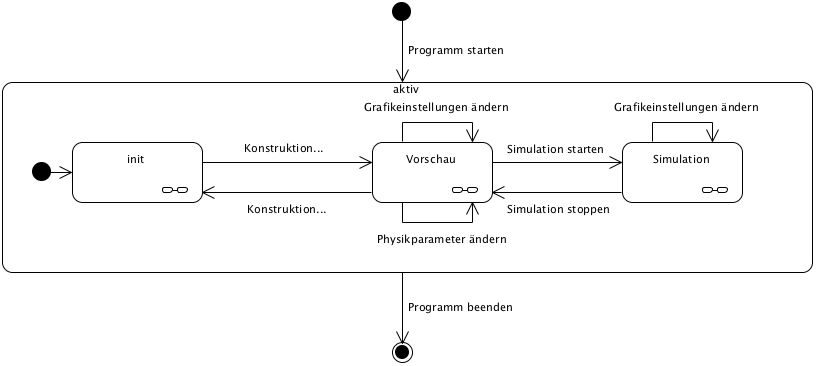
\includegraphics[width=\linewidth]{bilder/StateChart_GUI}
\caption{Statechart für die \textit{Benutzeroberfläche}}
\end{figure}

\subsection{Simulator}
Der Simulator ist das Kernstück der Anwendung und repräsentiert das Zusammenspiel aus physikalischen Berechnungen
und grafischer Darstellung der Achterbahnfahrt. Die Zustandswechsel des Simulators verlaufen synchron mit 
denen der Benutzeroberfläche. Nach dem Starten des Programms befindet sich der Simulator in einem Initialzustand,
der noch keine Simulation repräsentiert. Durch das Befüllen mit der Spezifikation der Achterbahn wird
eine Simulation instanziert und zur Vorschau gebracht. Mit dem Start der Simulation werden in diskreten Zeitschritten
die aktualisierten physikalischen Daten eingelesen und zur Veränderung der Kameraposition verwendet. Durch das
Stoppen der Simulation kehrt auch der Simulator wieder in die Vorschau zurück.

\subsection{3D-Anzeige}
Die 3D-Anzeige dient zur Visualisierung der Achterbahnfahrt, also zur Darstellung der Bahn als 3D-Modell aus
einer vorgegebenen Kameraperspektive. Vor der Bereitstellung eines konkreten Achterbahnmodells befindet sich
die Anzeige in einem Initialzustand, in welchem es in Ermangelung von Daten nicht möglich eine Szene darzustellen. 

\begin{figure}
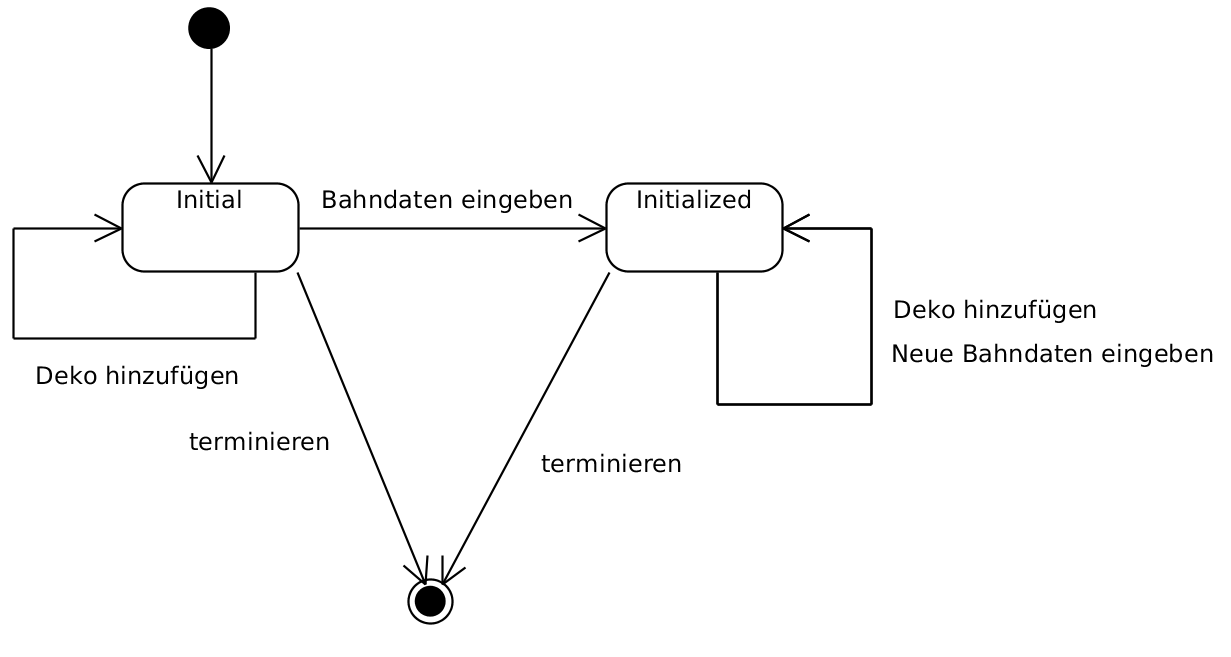
\includegraphics[width=\linewidth]{bilder/statechart_3dgraphics}
\caption{Statechart für die \textit{3D-Anzeige}}
\end{figure}

Durch Übergabe der Bahndaten kann die 3D-Anzeige die Achterbahn und deren Umgebung für die Anzeige vorberechnen.
Aber erst nach dem Start der Simulation, werden regelmäßig Bilder berechnet und angezeigt. Aus Sicht der 3D-Anzeige
können nach der Beladung jederzeit Änderungen wie Einfügen von Dekoration oder Anpassen der grafischen Einstellungen
vorgenommen werden, ohne das eine Zustandsänderung erforderlich wäre. Allerdings müssen innerhalb des Render-Vorgangs
eines einzelnen Bildes die Einstellungen unverändert bleiben, damit eine saubere Kommunikation mit dem 3D-Hardwarekontext
gewahrt bleibt.

\subsection{Physik und Mathematik}

Die physikalischen Berechnungen des Achterbahnsimulators folgen den Gesetzen der Newtonschen Mechanik für die Bewegung
eines Massenpunktes auf einer vorgegebenen Bahn im Gravitationsfeld der Erde. Berechnet wird die Bahnkurve als Lösung
einer gewöhnlichen Differentialgleichung mit vorgegebenen Anfangswerten. Die Lösung erfolgt nach einem numerischen
Verfahren, welches über die Zeit integriert.

Entsprechend wird der Zustand des Systems nach der Initialisierung mit den Bahndaten und den Anfangswerten von Zeitpunkt
zur Zeitpunkt weiterentwickelt, bis die Simulation (z.B. über Programmende) beendt wird.

Für die Berechnung der Bahnkurven kommen eine Reihe von Hilfsmethoden zum Einsatz. Diese Routinen sind zustandslos und
besitzen keinen eigenen Lebenszyklus.

\begin{figure}
\includegraphics[width=\linewidth]{bilder/statechart_physics}
\caption{Statechart für die \textit{Physik}}
\end{figure}
                % Kapitel 1
% Kapitel 2 mit den entsprechenden Unterkapiteln
% Die Unterkapitel können auch in separaten Dateien stehen,
% die dann mit dem \include-Befehl eingebunden werden.
%-------------------------------------------------------------------------------
\chapter{Erfüllung der Kriterien}

Nachfolgend wird beschrieben, wie die einzelnen Kriterien des Pflichtenheftes
erfüllt werden und worauf geachtet wird.  Es ist dabei explizit auf die
definierten Kriterien des Pflichtenheftes zu verwiesen.
\section{Musskriterien}

Die folgenden Kriterien sind unabdingbar und müssen durch das Produkt erfüllt
werden:
\begin{description}
	\item[/M10/] Die physikalisch korrekte Wiedergabe des Fahrverhaltens der Achterbahn aus der Perspektive eines Fahrgastes wird durch eine in Echtzeit modellierte Bahn und eine Umgebung visualisiert. Es wird darauf geachtet, dass der Boden bei z=0 ist wie in /F510o/ des Pflichtenheftes beschrieben.
	\item[/M20/] Berechnung und Darstellung der Bahn erfolgt in Echtzeit
	\item[/M30/] Darstellung eines ebenen Bodens als Grundfläche wie in /F521o/ des Pflichtenheftes beschrieben.
	\item[/M40/] Darstellung zweier parallel verlaufender Schienen mit mindestens zwei Querbalken pro Streckenabschnitt
	\item[/M50/] Eine 2D- Visualisierung der Beschleunigung wird in der 2D-GUI angezeigt und wird in einem Textfeld ausgewertet wie in /F532/ des Pflichtenheftes beschrieben.
\end{description}

\section{Wunschkriterien}
Die Erfüllung folgender Kriterien für das abzugebende Produkt wird angestrebt:

\begin{description}
	\item[/W10/] Berechnung der Luft- und Bahnreibung wie in /F510o/ des Pflichtenheftes beschrieben.
	\item[/W20/] Erfassung von Bremsvorgängen wie in /F500/ beschrieben.
	\item[/W30/] Berücksichtigung der Beschleunigungskräfte durch Wagen und Passagiere, wie in /F510o/ beschrieben.
	\item[/W40/] Bei der Visualisierung von Stützbalken ist darauf zu Achten, dass keine Stützbalken durch die Bahn gehen wie in /F521o/ des Pflichtenheftes beschrieben.
	\item[/W50/] Die Darstellung der Umgebung mit Gebäuden, Bepflanzung und Himmel verschönern die Simulation und bieten dem Benutzer außerdem Orientierung. Wichtig dabei ist, dass keine Dekoration durch die Bahn geht, wie in /F521o/ des Pflichtenheftes beschrieben. 
	\item[/W60/] Die Verstellbare Kamera zwischen Innenansicht und Außenperspektive wird über eine Scrollbar in der 2D-GUI eingestellt und sofort geändert, wie in /F533o/ des Pflichtenheftes erklärt.
	\item[/W70/] Der Achterbahnwagen wird modelliert und ist bei der Außenperspektive sichtbar. Bei der Innenansicht ist der Wagen nicht zu sehen.
	\item[/W80/] Implementierung einer Zeitrafferfunktion mit der Möglichkeit zum Vor- und Zurückspulen, wie in /F522o/ des Pflichtenheftes beschrieben
	\item[/W90/] Implementierung einer Aufnahmefunktion für Einzelbilder und Filme wie in /F400o/ des Pflichtenheftes beschrieben.
\end{description}

\section{Abgrenzungskriterien}
Folgende Funktionalitäten werden nicht durch das Produkt, sondern wie folgt
beschrieben anderweitig erfüllt:
\begin{description}
	\item[/A10/] Keine eigenständige Funktionalität zum Erstellen oder Ändern der Achterbahnen
	\item[/A20/] Keine Simulation der statischen und dynamischen Belastungen auf das Achterbahntragwerk
	\item[/A30/] Keine Überprüfung der Tragfähigkeit des Gerüstes
	\item[/A40/] Keine Berücksichtigung äußerlicher Einflüsse auf die Achterbahn
	\item[/A50/] Keine Passagiere
	\item[/A60/] Keine Untersuchung von Sicherungsmaßnahmen
\end{description}      % Kapitel 2
% Kapitel 3 mit den entsprechenden Unterkapiteln
% Die Unterkapitel können auch in separaten Dateien stehen,
% die dann mit dem \include-Befehl eingebunden werden.
%-------------------------------------------------------------------------------
\chapter{Implementierungsentwurf}

In diesem Kapitel werden die Implementierungsdetails für die Umsetzung des
Grobentwurfs vorgestellt. Gegenüber letzterem werden neben den Schnittstellen
auch die Implementierungen spezifiziert. Die Abbildungen zeigen die 
Klassenhierachie in den jeweiligen Paketen. Aus Gründen der Übersichtlichkeit
wird in den Implementierungen auf die Auflistung der Operationen der Schnittstellen
verzichtet.

\begin{figure}[!h]
	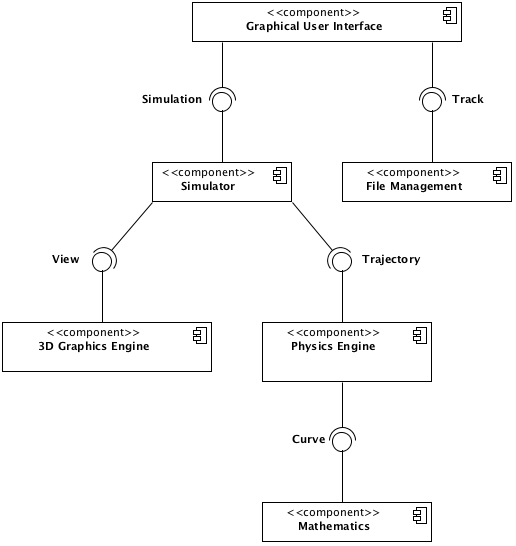
\includegraphics[width=0.8\linewidth]{bilder/components.png}
\caption{Komponentendiagramm}
\end{figure}


\section{Gesamtsystem}
Fügen Sie hier bitte das Komponentendiagramm aus dem Grobentwurf ein und
erläutern Sie kurz die Funktionen der Komponenten.
%%%%%%%%%%%%%%%%%%%%%%%%%%%%%%%%%%%%%%%%%%%%%%%%%%%%%%%%%%%%
\section{Implementierung von Komponente
         <ID aus Grobentwurf>: <Komponentenname>:}

Beschreiben Sie hier bitte die Implementierung der Komponente. Erläutern Sie
bitte dabei, welche Entwurfsmuster und Bibliotheken Sie verwenden. Die
Implementierung wird dabei durch Klassendiagramme dokumentiert.

\subsection{Paketdiagramm}
\subsection{Erläuterung}

Die verwendeten Attribute, Aufgaben und Kommunikationspartner sind für jede
Klasse kurz zu erläutern. Die ankommenden Nachrichten beziehen sich dabei auf
die Sequenzdiagramme der Feinanalyse im Grobentwurf und stellen meist
aufzurufende Methoden der Klasse dar.  Reine get- / set-Methoden oder
Bibliotheksfunktionen brauchen nicht aufgeführt zu werden.


%%%%%%%%%%%%%%%%%%%%%%%%%%%%%%%%%%%%%%%%%%%%%%%%%%%%%%%%%%%%
\section{Implementierung von Komponente
         xx: 3D-Anzeige:}

Die  3D-Anzeige-Komponente übernimmt die dreidimensionale Visualisierung der Achterbahn
mit Gerüst und Umgebung.Sie kapselt die allgemeinen gehaltenen Funktionen der eingesetzten
Grafikbibliothek JMonkeyEngine und stellt eine einfache Schnittstelle für das Befüllen 
der virtuellen Welt mit Achterbahnkomponenten sowie zur Steuerung der Kamerafahrten 
entlang der befahrenen Strecke zur Verfügung.

\textbf {Dieser Bereich ist noch nicht entgültig fertig,bedarf einer Überarbeitung und steht zur Diskussion!}

\begin{figure}
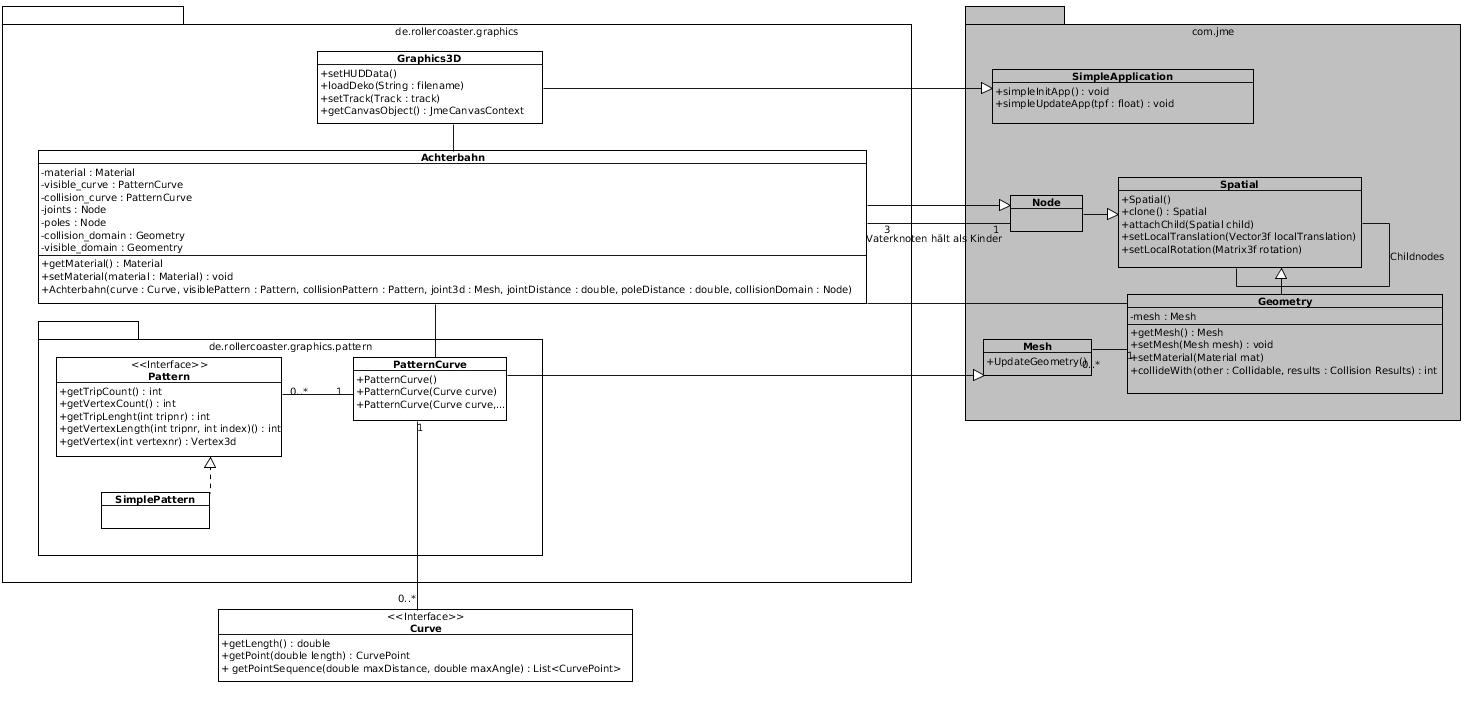
\includegraphics[width=\linewidth]{bilder/klassendiagramm_004}
\caption{Klassendiagramm Achterbahn}
\end{figure}

Die JMonkeyEngine stellt eine Scenegraphenstruktur über Spatial zur Verfügung die hier kurz skizziert wird. Die Subklassen Geometry als Meshcontainer und Node als Strukturelement werden von unserer Hauptklasse Achterbahn 
zur Speicherung und Ordnung der Geometrieelemente verwendet. PatternCurve ist eine Klasse die ein Pattern entlang einer Curve extrudiert.

\begin{figure}
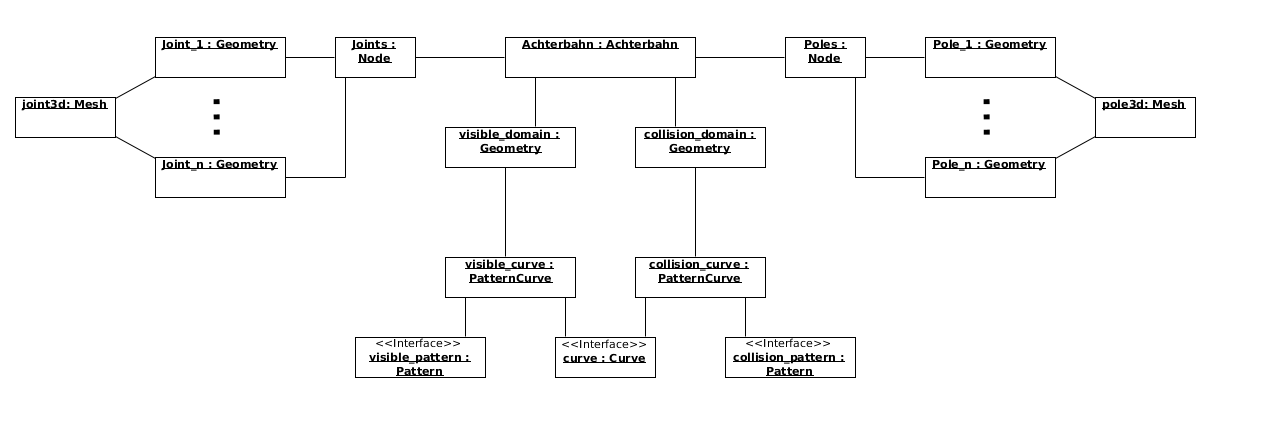
\includegraphics[width=\linewidth]{bilder/objektdiagramm_004}
\caption{Objektdiagramm Achterbahn}
\end{figure}

Im wesentlichen hält die Achterbahn 4 Knoten. Unter joints hängen alle n Geomentrien die auf die gleiche Mesh zeigen und die Verbindungsstücke der Bahn erzeugen. Das Konzept erlaubt, dass in jedem Geometry eigene Rotation und 
Translation gesetzt werden, sodass die Mesh an unterschiedlichen Orten im 3D-Raum gezeichnet wird, ohne jedoch die Mesh im Speicher vollständig kopieren zu müssen. Poles enthält die Stützpfeiler der Bahn und ist analog strukturiert.
Die Schienen werden in der visible\_domain durch eine PatternCurve erzeugt. In der collision\_domain liegt eine zweite PatternCurve, die ein BoundingVolume um die Bahn definiert um Kollisionen mit bereits geladener oder neu zu ladener
Dekoration zu erkennen. Dieses BoundingVolume wird außerdem dazu verwendet die Stützpfeiler zu generieren, ohne dass diese in durch die Bahn ragen.

\begin{figure}
  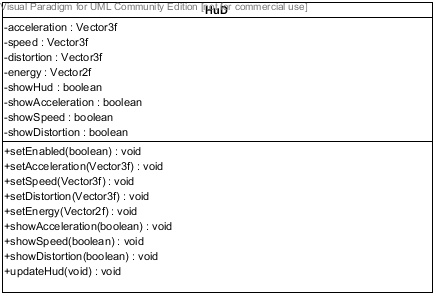
\includegraphics[width=0.8\linewidth]{bilder/HuD.png}
 \caption{Head up Display}
\end{figure}
Auf die von der JMonkeyengine bereitgestellte Zeichenfl"ache wird ein \textsl{Head up Display} projeziert. Dieses diehnt dazu dem Benutzer einen schnellen 
"Uberblick "uber den  aktuellen Status der Simulation zu erlauben, ohne erst die Messwerte numerisch auswerten zu m"ussen. Dem \textsl{HuD} können verschiedene Werte zur
Anzeige "ubergeben werden.

\subsection{Paketdiagramm}
\subsection{Erläuterung}

Die verwendeten Attribute, Aufgaben und Kommunikationspartner sind für jede
Klasse kurz zu erläutern. Die ankommenden Nachrichten beziehen sich dabei auf
die Sequenzdiagramme der Feinanalyse im Grobentwurf und stellen meist
aufzurufende Methoden der Klasse dar.  Reine get- / set-Methoden oder
Bibliotheksfunktionen brauchen nicht aufgeführt zu werden.

%%%%%%%%%%%%%%%%%%%%%%%%%%%%%%%%%%%%%%%%%%%%%%%%%%%%%%%%%%%%
\section{Implementierung von Komponente
         <ID aus Grobentwurf>: Benutzeroberfläche:}

Die grafische Benutzeroberfläche übernimmt die Interaktion zwischen dem Benutzer und
der Simulation. Dazu gehört die Steuerung des Hauptmenüs, des Dateidialoges und
des Optionen-Dialogs. Die aus der Dateiverwaltung ausgelesenen Achterbahn-Kurven 
werden an den Simulator zur Darstellung übergeben. Die Nutzeraktionen bezüglich des
Simulationsablaufes werden durchgereicht. Die Benutzeroberfläche lässt sich über
Änderungen am physikalische Zustand des Achterbahnwaagens informieren und stellt
wichtige Daten grafisch dar.

\subsection{Paketdiagramm}
\subsection{Erläuterung}

Die verwendeten Attribute, Aufgaben und Kommunikationspartner sind für jede
Klasse kurz zu erläutern. Die ankommenden Nachrichten beziehen sich dabei auf
die Sequenzdiagramme der Feinanalyse im Grobentwurf und stellen meist
aufzurufende Methoden der Klasse dar.  Reine get- / set-Methoden oder
Bibliotheksfunktionen brauchen nicht aufgeführt zu werden.

%%%%%%%%%%%%%%%%%%%%%%%%%%%%%%%%%%%%%%%%%%%%%%%%%%%%%%%%%%%%
\section{Implementierung von Komponente
         <ID aus Grobentwurf>: Dateiverwaltung:}

Die Dateiverwaltungs-Komponente übernimmt das Einlesen der Achterbahn-Spezifikationen 
aus den vom Editor bereitgestellten XML-Dateien. Alle speziellen Eigenheiten des
eingesetzten Serialisierung-Schema werden gekapselt. Den übrigen Komponenten wird 
lediglich eine glatte Raumkurve und ein Satz einfach auslesbarer Parameter zur Verfügung
gestellt.

\subsection{Paketdiagramm}

\begin{figure}
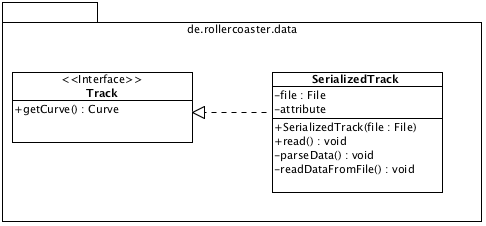
\includegraphics[width=\linewidth]{bilder/Data}
\caption{Daten}
\end{figure}

\subsection{Erläuterung}

Erläuterung folgt

%%%%%%%%%%%%%%%%%%%%%%%%%%%%%%%%%%%%%%%%%%%%%%%%%%%%%%%%%%%%
\section{Implementierung von Komponente
         <ID aus Grobentwurf>: Mathematik}

Die Mathematik-Komponente stellt Routinen zur näherungsweisen Berechnung
von Beziérkurven, dem Lösen von gewöhnlichen Differentialgleichungen 
(Anfangswertproblemen) und Algorithmen zum Lösen von linearen Gleichungssystemen
zur Verfügung. Dadurch ist es möglich, aus einer über Stützstellen definierte 
Achterbahn in eine glatte Raumkurve umzurechnen und die Bewegung auf
der Bahnkurve durch numerische Integration zu bestimmen.

\subsection{Paketdiagramm}

\begin{figure}
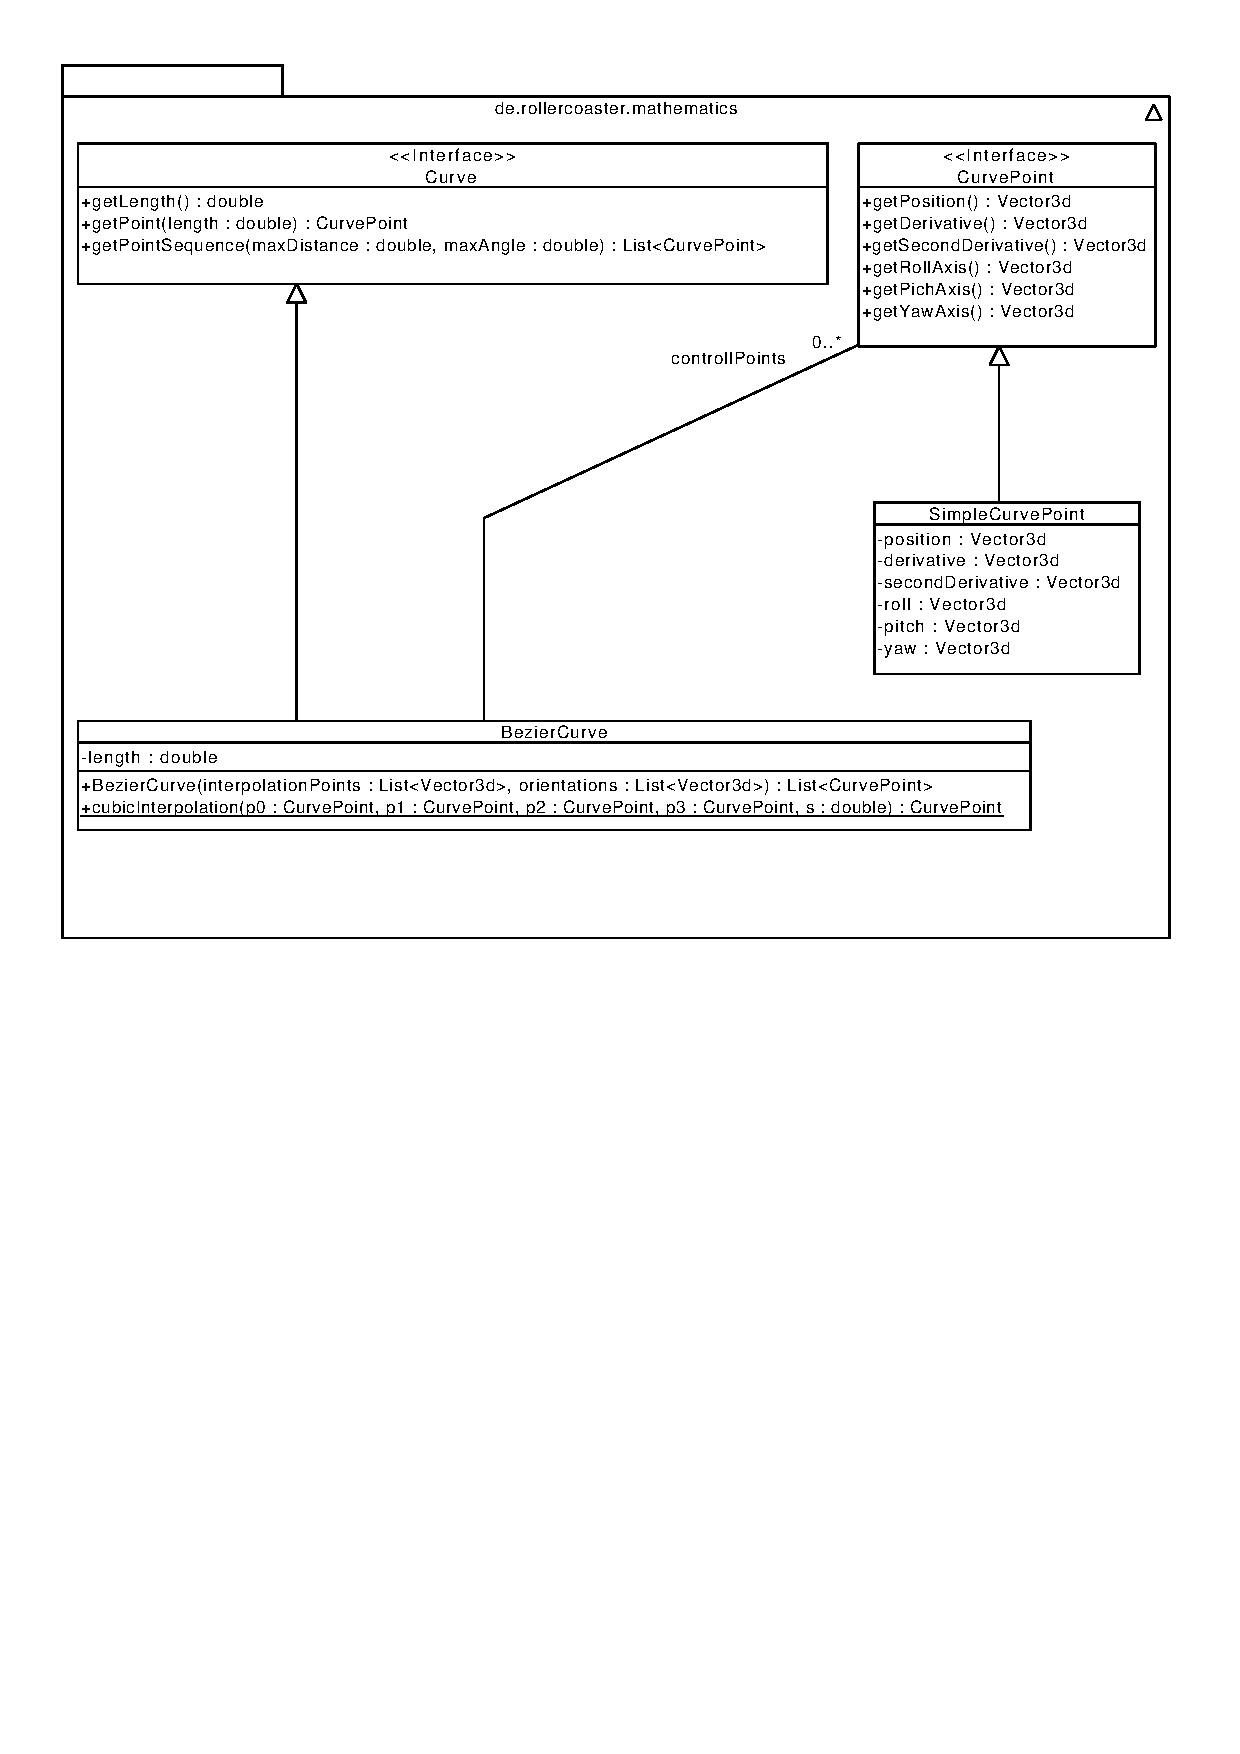
\includegraphics[width=\linewidth]{bilder/Mathematics}
\caption{Mathematik (Raumkurven)}
\end{figure}
\begin{figure}
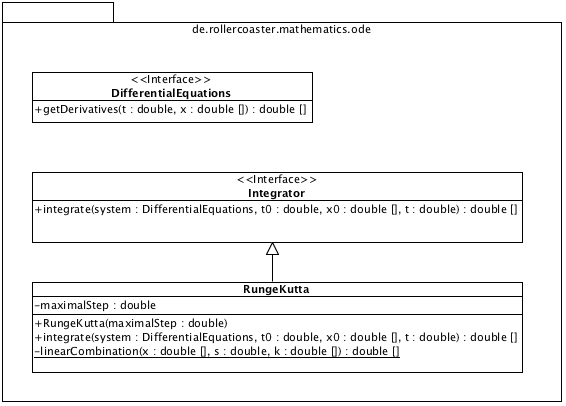
\includegraphics[width=\linewidth]{bilder/Mathematics_ODE}
\caption{Mathematik (Diffentialgleichungen)}
\end{figure}

\subsection{Erläuterung}

Erläuterung folgt

%%%%%%%%%%%%%%%%%%%%%%%%%%%%%%%%%%%%%%%%%%%%%%%%%%%%%%%%%%%%
\section{Implementierung von Komponente
         <ID aus Grobentwurf>: Physik:}

In der Physik-Komponente erfolgt die Berechnung der Achterbahnbewegung. Dazu wird
die Bewegung eines Massenpunktes auf der von Außen vorgegebenen Raumkurve
nach den Gesetzen der klassischen Mechanik bestimmt. Die Berechnung erfolgt
durch numerisches Lösen einer gewöhnliche Differentialgleichung, welche von der
Physik-Komponente repräsentiert und von der Mathematik-Komponente integriert wird.
Für jeden Zeitschritt wird der Zustand des Massenpunktes aktualisiert und an die
übergeordneten Komponenten weitergereicht.

\subsection{Paketdiagramm}
\begin{figure}
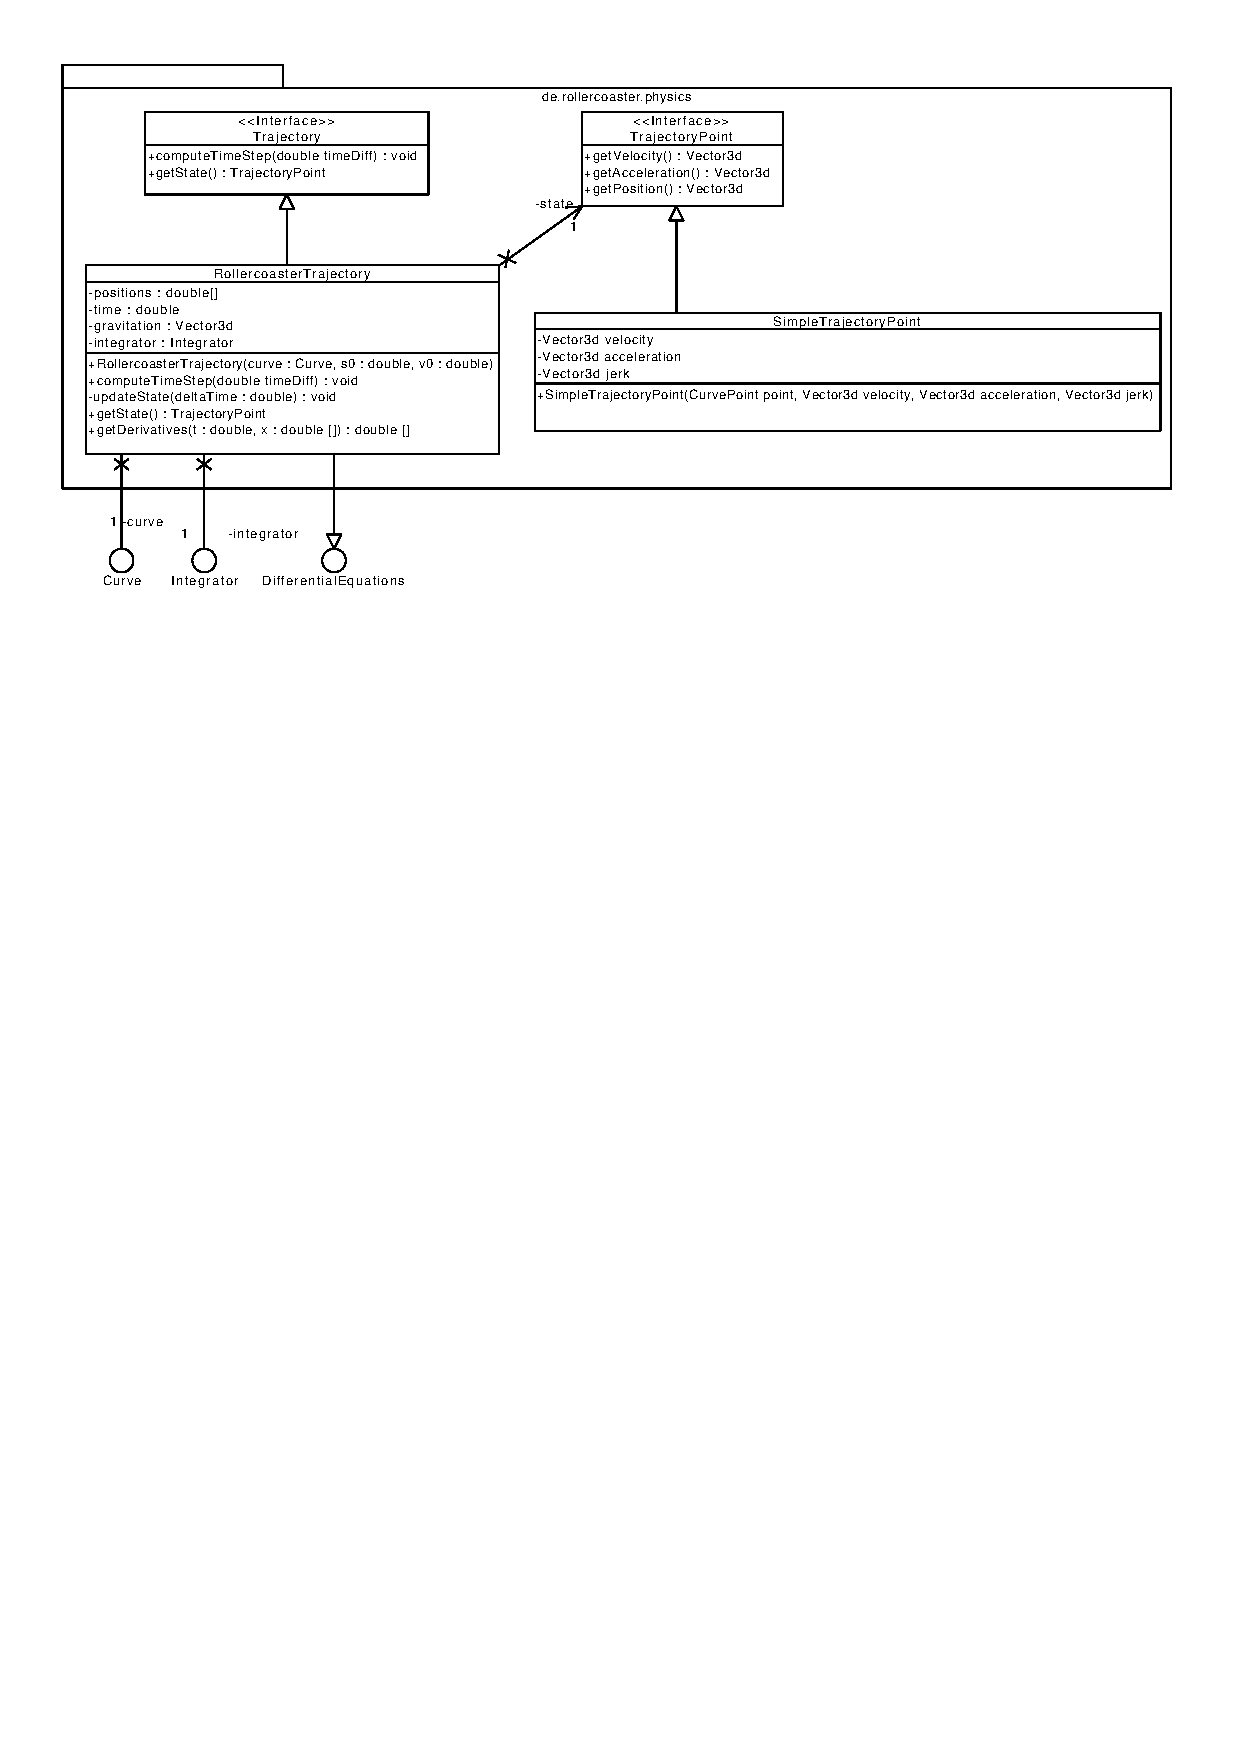
\includegraphics[width=\linewidth]{bilder/Physics}
\caption{Physik}
\end{figure}

\subsection{Erläuterung}

Erläuterung folgt


%%%%%%%%%%%%%%%%%%%%%%%%%%%%%%%%%%%%%%%%%%%%%%%%%%%%%%%%%%%%
\section{Implementierung der Komponente Simulator:}

Die Simulator-Komponente steht im Kern der Anwendung. Sie ist für die Steuerung der
Achterbahnbewegung verantwortlich ist und koordieniert zwischen der physikalischen 
Berechnung und der grafischen Umsetzung. Dieser Komponente werden eine konkrete 
Raumkurve für den Bahnnverlauf und die physikalischen Parameter übergeben, welche
als Simulation umgesetzt werden sollen. Die Komponente wird über eine 
Endlosschleife (``render loop'') im Gang gehalten. Aus Implementierungsgründen wird
die Steuerung der Zeitschritte über die Grafikkomponente angetrieben und von der
Simulation nur verteilt.

\subsection{Paketdiagramm}
\begin{figure}
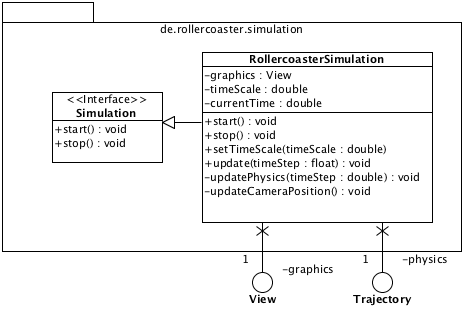
\includegraphics[width=\linewidth]{bilder/Simulation}
\caption{Simulation}
\end{figure}

\subsection{Erläuterung}

Erläuterung folgt
  % Kapitel 3
% Kapitel 4 mit den entsprechenden Unterkapiteln
% Die Unterkapitel können auch in separaten Dateien stehen,
% die dann mit dem \include-Befehl eingebunden werden.
%-------------------------------------------------------------------------------
\chapter{Datenmodell}
Falls in der Anwendung bestimmte Daten dauerhaft gespeichert werden, so sind
die entsprechenden Entities und Beziehungen hier darzustellen und zu erläutern.
Dies ist insbesondere relevant, falls der Einsatz einer (relationalen)
Datenbank geplant ist.

\section{Diagramm}

Eigenes ER-Modell einsetzen
\section{Erläuterung}
Die Tabelle ist um so viele Einträge zu erweitern, wie es Entities im obigen
ER-Modell gibt. Für jedes Entity sind so viele Einträge in der
Beziehungs-Subtabelle einzufügen, wie es Beziehungen zu diesem Entity gibt.


\begin{tabular}[ht]{|l|c|}
  \hline
  Entität & Beziehungen\\
  \hline\hline
  <Entity … ID>:  & Name der Beziehung |  Kardinalität\\
  \hline\hline\hline
  <Bezeichnung> & <Name der Beziehung> | <Kardinalität>\\
  \hline
\end{tabular}
              % Kapitel 4
%% Kapitel 5
%-------------------------------------------------------------------------------
\chapter{Serverkonfiguration}
Sollte ein Server (z. B. Tomcat) für die Bearbeitung und Nutzung des Produktes
erforderlich sein, so ist hier dessen Konfiguration zu beschreiben. Dies
geschieht durch explizite Nennung aller Konfigurationsdateien und notwendiger
Einträge.

      % Kapitel 5
% Kapitel 9
%-------------------------------------------------------------------------------

\chapter{Glossar}
Hier werden Fachbegriffe erklärt.
  

%------Ende des Dokumentes------------------------------------------------------
\end{document}
